\begin{center}
	\begin{tikzpicture}
	\node[anchor=south west,inner sep=0] (image)  at (0,0) {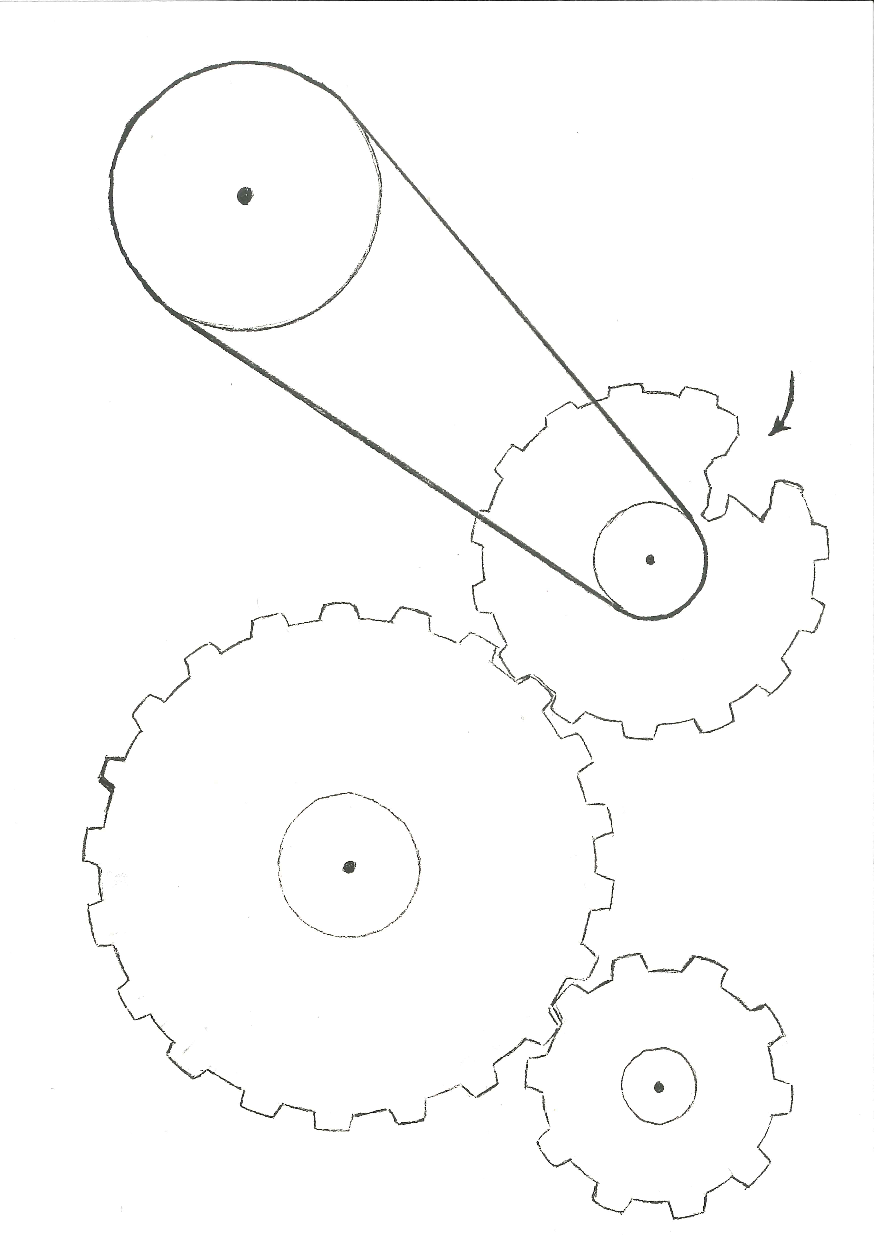
\includegraphics[trim={2mm, 2mm, 2mm, 2mm}, clip, angle=180, width=0.995\pagewidth]{scans/pan-5.pdf}};
	
	
	\begin{scope}[x={(image.south east)},y={(image.north west)}]
	\if\helplines1
	\draw[help lines,xstep=.1,ystep=.1] (0,0) grid (1,1);
	\fi

	\node[align=center, anchor=south west, text width=0.3\pagewidth](en) at (0.05, 0.62) {\english{Understanding proteins help us understand how the machines break - what we call disease - and how to fix it, ie., heal.}};
	\node[align=center, anchor=north west, text width=0.4\pagewidth](es) at (0.55, 0.48) {\spanish{Entender cómo funcionan las proteínas nos ayuda a entender cómo y por qué estas máquinas se estropean - lo que llamamos enfermedad - y cómo arreglarlas, es decir, curar.}};
	\end{scope}
	
	\end{tikzpicture}
\end{center}